\documentclass[12pt]{article}
\usepackage{geometry} 
\geometry{margin=1in}
\geometry{a4paper} 


\usepackage{textcomp}
\usepackage{booktabs}
\usepackage{array}
\usepackage{paralist}
\usepackage{verbatim} 
\usepackage{subfigure}
\usepackage{graphicx,caption}
\usepackage{placeins}
\usepackage{lipsum}
\usepackage{xcolor}
\usepackage{dcolumn}
\usepackage{sectsty}
\allsectionsfont{\sffamily\mdseries\upshape}
\usepackage{gensymb,amsmath,mathtools,amssymb}
\usepackage{flafter}
%\usepackage{parskip}
\usepackage[utf8]{inputenc}
\usepackage[english]{babel}
\usepackage{tocbibind}
\usepackage[toc,page]{appendix}
\captionsetup{width=\linewidth}
\usepackage{bm}
\usepackage{url}

\usepackage{tikz}
\usetikzlibrary{shapes, arrows}

\newcommand{\half}{\frac{1}{2}}


\graphicspath{{./figs/}}


\title{Short term plan for Systems}
\author{Devansh Agrawal\\ICLR Systems}
\date{October 26, 2019} 


\begin{document}

\maketitle


\section{Summary}

There are three major tasks that need to be completed in about the next week or two, and pretty much need to happen in parallel.

\begin{enumerate}
\item Define top level requirements in Valispace
\item Preliminary and semi-detailed sizing
\item Standard interface definition
\end{enumerate}

This document provides some guidance on why these are critical next steps, and on how we will go about doing these. 

\section{Define top level requirements}
\subsection{Why}
\begin{enumerate}
\item We can't let any high level requirements slip through the cracks of communication
\item All design decisions should be traceable to to the top level requirements
\end{enumerate}

\subsection{How}
There are a few types of top level requirements that need to be specified, and the first sub-level requirements can be specified from there. Every requirement must have a:
\begin{itemize}
\item \emph{owner} which is the person in charge of ensuring the requirement is met. 
\item \emph{description} which explains the requirements in words
\item \emph{success criteria} which is a specific rule that can be checked to see if the requirement is met (usually numeric)
\end{itemize}

The verification method for the requirement is needed if relevant. 

The top level requirements are derived from the competition:
\begin{enumerate}
\item COMP-SAFE-xxx: Competition safety requirements. These also include requirements on which tests need to be performed
\item COMP-PERF-xxx: Competition performance requirements. These include all the rocket performance requirements, including things like the launch rail velocity requirement or stability requirements.
\item COMP-TIME-xxx: Competition timeline requirements. These indicate all the deadlines from the compeititon, internal deadlines will be labelled differently.
\end{enumerate}

The xxx refers to the requirement ID number. 

From these competition requirements, all internal requirements should be derived. 

We will define these based on which system they are relevant to, and the breakdown of subsystems is defined in the next section. 

From here, the responsible engineers list should also be defined, which includes exact specification of which person is incharge of which components and which interfaces, to (again) prevent details from being missed in communication. 


\section{Preliminary and semi-detailed sizing}


\subsection{Why}

Most teams have not started a detailed component design as they are unaware of parameters from other teams. The initial sizing doc provides a decent estimate on the parameters, but now detailed sizing for each component must be carried out. 

Seeing that we don't have much time, this is roughly a mashup of both the preliminary and detailed sizing of Sporadic Impulse. 

\subsection{How}

\begin{enumerate}
\item Define most critical parameters and their relationships on valispace based on the initial sizing. At the same time, define these in openrocket 
\item  Perform a more detailed baseline estimation of the size of each component, working with the team members to produce accurate bounds on system parameters. 
\item  Continuously feed back into valispace such that the design can stay upto date. 
\item Ensure all top level requirements are still being met. 
\item Perform more detailed sizing of the components. 
\end{enumerate}


Initially, we can start by spec-ing a cardboard body tube and nothing too fancy in general. All the embellishments, like generative design or special manufactured components can either be ignored at this stage, or estimated as some percentage reduction in mass (or whichever relevant parameter you have). Please don't forget which assumptions you have made, and to go back and correct them later. 

\section{Standard Interfaces}

\subsection{Why}
To reduce design time and communication, we must define the basic standard interfaces between teams. Teams are free to modify them later but must agree upon it. Essentially we want to avoid scenarios where we are trying to fit an M4 screw into an M5 hole that is 0.2 mm too far to the left. 

\subsection{How}

The key interfaces we need to define are:  (1) mechanical, (2) electrical

\begin{enumerate}
\item Understand the relevant load paths, and figure out where the mechanical connections should be
\item Design it to allow for easy changes down the line - think lego rather than 3d printing - it should require minimal effort to change the rocket later and 3d printing a new mount isnt really a 'quick' solution - it requires about a day to do, compared to minutes if you can just unscrew something and screw it in somewhere else. 
\item reduce the number of different types of screws or mountings there are 
\item dont forget about electrical paths
\end{enumerate}








\section{Additional Stuff: Fusion-Valispace-OpenRocket-API}

\subsection{Why}

Soon, we will be straddling at least three different environments - Valispace (where we store the parameters of the rocket), Fusion (where the detailed design of the rocket is) and OpenRocket (where much of the simulation and verification tools are. 

These need to be in sync, and the best way to do this is probably using an API where we can run a script, and it would sync across the three platforms. 

Specifically the interactions we need are (in order of priority):
\begin{enumerate}
\item \emph{Valispace $\rightarrow$ Fusion}

Valispace has the dimensions and parameters of some components that are subject to change, we need these parts to get updated in Fusion. 

\item \emph{ Fusion $\rightarrow$ Valispace}

Estimating the mass, centre of masses, moments of inertia and placement of components is tricky/too much additional work within Valispace. As such, it would be ideal if we can export these parameters from Fusion into Valispace. This requires the materials to be accurately described and correctly selected within Fusion.  It probably also requires everyone to agree on a standard coordinate system, which you should decide and stick to. There is no real reason to change this afterwards, and every subcomponent designed in Fusion should stick to this convention. Probably the easiest is to follow Fusions built in config, where $z$ points up the rocket, $x$ points to the right when looking at the rocket, ie. the $x-z$ plane defines the front face of the rocket (see the view cube below). Also important to define (for Valispace integration) is the reference location of each part, so the center of mass is measured relative to something, but this needs some more thought. 

%\FloatBarrier
\begin{figure}[htbp]
   \centering
   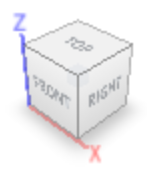
\includegraphics[width=0.2\linewidth]{view_cube.png}
   \caption{Standard orientation in Fusion}
   \label{fig:}
\end{figure}


\item \emph{ OpenRocket $\rightarrow$ Valispace}

OpenRocket should provide decent estimates on drag coefficient (need to be careful about the reference area used) the altitude reached and other such simulation results. Perhaps a small closed design loop can be created to select the boosters needed, but I think manual methods here will be sufficient and quite useful for understanding our rocket intuitively.  

\item \emph{ Fusion and Valispace $\rightarrow$ OpenRocket}

Using the parameters from both Fusion and Valispace, we somehow need to find the appropriate open rocket representation to be able to run the simulations. This means we need accurate masses in the right places, the right motor thrust curve. We should then be able to run the simulations. As far as I can tell, it will be tricky to run this simulation automagically unless we create a OpenRocket plugin (which isnt impossible). 


%FloatBarrier

\end{enumerate}

The figure below summarises this. 

%\FloatBarrier
\begin{figure}[htbp]
   \centering
   \includegraphics[width=0.7\linewidth]{software_workflow.eps}
   \caption{Basic information flow across our three main platforms}
   \label{fig:}
\end{figure}
%FloatBarrier


\subsection{How}

Fusion and Valispace both expose an API to input and export parameters, in a fairly (but not completely) trivial manner\footnote{Valispace has very poor filtering, and project hierarchy, Fusion's API must be run within their scripting menu}.  OpenRocket on the other hand does not, and the default \texttt{*.ork} file is not human-readable. The rocket can however be saved as a rocksim file, \texttt{*.rkt} file format, which stores the rocket and all its parameters as a XML format, explained in the rocksim documentation\footnote{ here is one version I found, there may be more: \url{https://www.apogeerockets.com/downloads/PDFs/Rocksim.pdf}}. Thus, in theory, we should be able to read parameters and simulation results, and the write straight to the file to see the result. The current best version of the rocket can be stored directly in Github, where the version tracking is done for you. 

Some automated way to run the simulations would be very helpful, especially for dispersion analysis, where we can modify each component by $\sim5\%$ and see how the apogee changes. We may even be able to use this interface to overwrite component mass and cog estimates, straight from valispace (which got it from fusion). 

All development of code should be done in Github. In the specific case of the Fusion API which must be stored in some weird directory of your computer, I would recommend linking that file to the Github tracker node. 

The exact implementation is to be determined based on what is feasible, but ideally there should be a function/bash script/button in Fusion that I can hit and everything gets updated. 


\section{Breakdown of System}

To avoid confusion, the  break down of  the entire system is specified here. This is distinct from the team layout, 

At the top level, there is either the \texttt{Rocket} or \texttt{Ground Support}, which contain:

\begin{enumerate}
\item Rocket
\begin{enumerate}
\item Payload
\item Avionics
\item Airframe
\item Recovery
\item Propulsion
\item Control Algorithm Software\footnote{need some thinking on whether it is appropriate here}.
\end{enumerate}
\item Ground Support
\begin{enumerate}
\item Storage and refuelling system
\item Telemetry and tracking equipment
\item Test equipment (including any relevant test stands and equipment needed for competition)
\item Transportation equipment (eg. boxes to store the rocket and its components, etc)
\item Tools and toolboxes 
\item etc. 
\end{enumerate}
\end{enumerate}

The  further breakdown is not specified here. In Valispace, we shall keep the \texttt{rocket} object not as a parent, but as a separate component. This is simply for convenience, as we don't want to have to refer to valis as \texttt{rocket.avionics.mass} but simply as \texttt{avionics.mass}. Ground support equipment should still be kept separate. 



\end{document}























